% !TEX root = sum1.tex
\section{Results}
We carried out several experiments, including comparing the running time of decomposition and integer programming, comparing the number of people served using the feasible seat planning and integer programming methods, analyzing different policies, evaluating the impact of implementing social distancing.

% assessing the results for different numbers of people in each period and finally investigating the impact of seat layout on the number of served people.


\subsection{Running time of Benders Decomposition and IP}\label{Bender_IP}
% At first, we compare the running time of these two methods. 

The running times of solving SSP directly and solving the LP relaxation of SSP with Benders decomposition are shown in Table \ref{tab_1}.

\begin{table}[ht]
  \centering
  \scriptsize
  \caption{Running time of Decomposion and IP}\label{tab_1}
  \begin{tabular}{|l|l|l|l|l|l|l|}
  \hline
  \# of scenarios & demands & \# of rows & \# of groups & \# of seats & running time of IP(s) & Benders (s) \\
  \hline
  1000  & (150, 350) & 30 & 8 & (21, 50) & 5.1  & 0.13 \\
  5000  &            & 30 & 8 &         & 28.73 & 0.47  \\
  10000 &            & 30 & 8 &         & 66.81  & 0.91 \\
  50000 &            & 30 & 8 &         & 925.17 & 4.3 \\
  \hline
  1000  & (1000, 2000) & 200 & 8 & (21, 50) & 5.88 & 0.29 \\
  5000  &              & 200 & 8 &          & 30.0 & 0.62 \\
  10000 &              & 200 & 8 &          & 64.41 & 1.09 \\
  50000 &              & 200 & 8 &          & 365.57 & 4.56\\
  \hline
  1000  & (150, 250) & 30 & 16 & (41, 60) & 17.15  & 0.18 \\
  5000  &            & 30 & 16 &          & 105.2  & 0.67 \\
  10000 &            & 30 & 16 &          & 260.88 & 1.28 \\
  50000 &            & 30 & 16 &          & 3873.16 & 6.18 \\
  \hline
  \end{tabular}
\end{table}

The parameters in the columns of the table are the number of scenarios, the range of demands, running time of integer programming, running time of Benders decomposition method, the number of rows, the number of group types and the number of seats for each row, respectively. 

Take the first experiment as an example, the scenarios of demands are generated from (150, 350) randomly, the number of seats for each row is generated from (21, 50) randomly.
% about 1000 seats.

% The second one:
% The number of seats for each row L is generated from (21, 50) randomly, about 7000 seats.
% The scenarios of demands are generated from (1000, 2000) randomly.

% The third one:
% The number of seats for each row L is generated from 41-60 randomly, about 1500 seats.
% The scenarios of demands are generated from (150, 250) randomly.

\subsection{Seat Planning Composed of Full or Largest Patterns versus IP Solution}
An arrival sequence can be expressed as $\{y_{1}, y_{2}, \ldots, y_{T}\}$. Let $N_{i} = \sum_{t} I(y_t = i)$, i.e., the number of times group type $i$ arrives during $T$ periods. Then the scenarios, $(N_1, \ldots, N_{M})$, follow a multinomial distribution, $$p\left(N_1, \ldots, N_{M} \mid \mathbf{p}\right)=\frac{T !}{N_{1}!, \ldots, N_{M}!} \prod_{i=1}^{M} p_{i}^{N_i}, T = \sum_{i=1}^{M} N_{i}.$$

It is clear that the number of different sequences is $M^{T}$. The number of different scenarios is $O(T^{M-1})$ which can be obtained by the following DP.

Use $D(T, M) $ to denote the number of scenarios, which equals the number of different solutions to $x_{1}+\ldots + x_{M} = T, \mathbf{x} \geq 0$. Then, we know the recurrence relation $D(T, M) = \sum_{i= 0}^{T} D(i, M-1)$ and boundary condition, $D(i,1) = 1$. So we have $D(T,2) = T+1$, $D(T,3) = \frac{(T+2)(T+1)}{2}, D(T,M) = O(T^{M-1})$. The number of scenarios is too large to enumerate all possible cases. Thus, we choose to sample some sequences from the multinomial distribution.

Then, we will show the seat planning has a close performance with IP when considering group-type control policy.

\begin{table}[ht]
    \caption{Feasible seat planning versus IP solution}
    \begin{tabular}{|l|l|l|l|l|l|l|}
    \hline
    \# samples & T & probabilities & \# rows & people served by decomposition & people served by IP \\
    \hline
    1000  & 45  & [0.4,0.4,0.1,0.1] & 8 & 85.30 & 85.3 \\
    1000  & 50  & [0.4,0.4,0.1,0.1] & 8 & 97.32 & 97.32 \\
    1000  & 55  & [0.4,0.4,0.1,0.1] & 8 & 102.40 & 102.40  \\ % slow
    1000  & 60  & [0.4,0.4,0.1,0.1] & 8 & 106.70 & NA  \\
    1000  & 65  & [0.4,0.4,0.1,0.1] & 8 & 108.84 & 108.84 \\
    \hline
    1000  & 35  & [0.25,0.25,0.25,0.25] & 8 & 87.16 & 87.08 \\
    1000  & 40  & [0.25,0.25,0.25,0.25] & 8 & 101.32 & 101.24 \\
    1000  & 45  & [0.25,0.25,0.25,0.25] & 8 & 110.62 & 110.52 \\
    1000  & 50  & [0.25,0.25,0.25,0.25] & 8 & 115.46 & NA \\
    1000  & 55  & [0.25,0.25,0.25,0.25] & 8 & 117.06 & 117.26 \\
    \hline
    5000  & 300  & [0.25,0.25,0.25,0.25] & 30 & 749.76 & 749.76 \\
    5000  & 350  & [0.25,0.25,0.25,0.25] & 30 & 866.02 & 866.42 \\
    5000  & 400  & [0.25,0.25,0.25,0.25] & 30 & 889.02 & 889.44 \\
    5000  & 450  & [0.25,0.25,0.25,0.25] & 30 & 916.16 & 916.66 \\
    \hline
    \end{tabular}
\end{table}

Each entry of people served is the average of 50 instances.
IP will spend more than 2 hours in some instances, as `NA' showed in the table.
The number of seats is 20 when the number of rows is 8, the number of seats is 40 when the number of rows is 30.

% We can find that the people served by Benders decomposition and IP under nested policy are close. But obtaining the near-optimal seat assignment will be faster.

% Thus, we can use the near-optimal seat assignment from the decomposition approach.

\subsection{Performances of Different Policies}
In this section, we compare the performance of four dynamic seat assignment policies to the optimal value, which can be obtained by solving the deterministic model after observing all arrivals. The policies under examination are the stochastic planning policy, DP Base-heuristic, bid-price policy and FCFS policy. The seat layout consists of 10 rows, each with 21 seats (including one dummy seat), and the group size can range up to 4 people. We conducted experiments over 60 to 100 periods to demonstrate the policies' performance under varying demand levels. We selected three probabilities to ensure that the expected number of people for each period is consistent. The table below displays the average of 200 instances for each number.

% dynamic programming based heuristic and booking limit control. Finally, we establish the FCFS policy as the benchmark.

\subsubsection{Booking Limit Control}
The booking limit control policy involves setting a maximum number of reservations that can be accepted for each group type. By controlling the booking limits, revenue managers can effectively manage demand and allocate inventory to maximize revenue.

In this policy, we replace the real demand by the expected one and solve the corresponding static problem using the expected demand. Then for every type of requests, we only allocate a fixed amount according to the static solution and reject all other exceeding requests. When we solve the linear relaxation of problem \eqref{deter_upper}, the aggregate optimal solution is the limits for each group type. Interestingly, the bid-price control policy is found to be equivalent to the booking limit control policy.

When we solve problem \eqref{deter_upper} directly, we can develop the booking limit control policy.

\begin{algorithm}[H]
  \caption{Booking limit control algorithm}
  \begin{description}
    \item[Step 1.] Observe the arrival group type $i$ at period $t = 1, \ldots, T$.
    \item[Step 2.] Solve problem \eqref{deter_upper} with $d_i^{t} = (T-t) \cdot p_i$ and $\mathbf{L}^{t}$, obtain the optimal solution, $x_{ij}^{*}$ and the aggregate optimal solution, $\mathbf{X}$.
    \item[Step 3.] If $X_{i} > 0$, accept the arrival and assign the group to row $k$ where $x_{ik} > 0$, update $\mathbf{L}^{t+1} = \mathbf{L}^{t} - n_i \mathbf{e}_{k}^{\top}$; otherwise, reject it, let $\mathbf{L}^{t+1} = \mathbf{L}^{t}$.
    \item[Step 4.] If $t \leq T$, move to next period, set $t = t+1$, go to step 2. Otherwise, terminate this algorithm.
  \end{description}
\end{algorithm}


% \begin{equation}
%   \begin{aligned}
%   \max \quad & \sum_{i=1}^{M}  \sum_{j= 1}^{N} (n_i- \delta) x_{ij} \\
%   \text {s.t.} \quad & \sum_{j= 1}^{N} x_{ij} \leq d_{i}, \quad i \in \mathcal{M}, \\
%   & \sum_{i} L_{ij} \leq L_j, \quad j \in \mathcal{N}, \\
%   & n_{i} x_{ij} - L_{ij} \leq 0, \quad i \in \mathcal{M}, j \in \mathcal{N} \\
%   & x_{ij} \geq 0, L_{ij} \geq 0, \quad i \in \mathcal{M}, j \in \mathcal{N}.
%   \end{aligned}
% \end{equation}

% \begin{equation}
%   \begin{aligned}
%   \min \quad & \sum_{i=1}^{M} d_i z_i + \sum_{j= 1}^{N} L_j \kappa_{j} \\
%   \text {s.t.} \quad & z_{i} + \beta_{ij} n_i \geq (n_i-\delta), \quad i \in \mathcal{M}, j \in \mathcal{N} \\
%   & \kappa_{j} - \beta_{ij} \geq 0, \\
%   & z_{i} \geq 0, i \in \mathcal{M}, \beta_{ij} \geq 0, j \in \mathcal{N}.
%   \end{aligned}
% \end{equation}

\subsubsection{Dynamic Programming Base-heuristic}
Since the original dynamic programming problem is too complex to solve directly, we can instead consider a simplified version of the problem, known as the relaxation problem. By solving the relaxation problem, we can make decisions for each group arrival based on the dynamic programming approach.

% Let $v_{r}^{*}$ and $v^{*}$ denote the optimal values of problem \eqref{relax_deter} and \eqref{deter_upper}, respectively. After relaxation, assume that each row has a capacity of $L$ seats, which can be filled. For each seperate row, the maximum number of empty seats in each row is $s$. Then, the total number of empty seats in $N$ rows is given by $Ns$. Therefore, the biggest difference between $v_{r}^{*}$ and $v^{*}$ is the number of people accommodated in the $Ns$ empty seats.
% The difference between them is zero only when the groups corresponding to the optimal solution of problem \eqref{relax_deter} can be accommodated in $N$ rows. The numerical results indicate that this is the case for most scenarios, which suggests that a DP-based approach can be used to solve the dynamic seat assignment problem after all groups have arrived.

Relax all rows to one row with the same capacity by $L = \sum_{j=1}^{N} L_j$. Let $u$ denote the decision, where $u(t) = 1$ if we accept a request in period $t$, $u(t) =0$ otherwise. Similar to the DP in section \ref{sec_dynamic}, the DP with one row can be expressed as:

$$V_{t}(L) = \mathbb{E}_{i \sim p} [\max_{u \in \{0,1\}} \{ {[V_{t+1}(L-n_i u)+ i u]}\}], L \geq 0, V_{T+1}(L) =0, \forall L$$

After accepting one group, assign it in some row arbitrarily when the capacity of the row allows.

\subsubsection{First Come First Served(FCFS) Policy}\label{largest_pattern}
For dynamic seat assignment for each group arrival, the intuitive but trivial method will be on a first-come-first-served basis. Each accepted request will be assigned seats row by row. If the capacity of a row is insufficient to accommodate a request, we will allocate it to the next available row. If a subsequent request can fit exactly into the remaining capacity of a partially filled row, we will assign it to that row immediately. Then continue to process requests in this manner until all rows cannot accommodate any groups.

\begin{table}[ht]
  \centering
  \caption{Performances of Different Policies}
  \begin{tabular}{|l|l|l|l|l|l|l|}
  \hline
   T & probabilities & SSP(\%) & DP1(\%) & Bid-price(\%) & Booking & FCFS(\%) \\
  \hline
   60  & [0.25, 0.25, 0.25, 0.25]  & 99.12 & 98.42 & 98.38 & 96.74 & 98.17 \\
   70  & [0.25, 0.25, 0.25, 0.25]  & 98.34 & 96.87 & 96.24 & 97.18 & 94.75 \\
   80  & [0.25, 0.25, 0.25, 0.25]  & 98.61 & 95.69 & 96.02 & 98.00 & 93.18 \\
   90  & [0.25, 0.25, 0.25, 0.25]  & 99.10 & 96.05 & 96.41 & 98.31 & 92.48 \\
   100 & [0.25, 0.25, 0.25, 0.25]  & 99.58 & 95.09 & 96.88 & 98.70 & 92.54 \\
   \hline
   60  & [0.25, 0.35, 0.05, 0.35]  & 98.94 & 98.26 & 98.25 & 96.74 & 98.62 \\
   70  & [0.25, 0.35, 0.05, 0.35]  & 98.05 & 96.62 & 96.06 & 96.90 & 93.96 \\
   80  & [0.25, 0.35, 0.05, 0.35]  & 98.37 & 96.01 & 95.89 & 97.75 & 92.88 \\
   90  & [0.25, 0.35, 0.05, 0.35]  & 99.01 & 96.77 & 96.62 & 98.42 & 92.46 \\
   100 & [0.25, 0.35, 0.05, 0.35]  & 99.23 & 97.04 & 97.14 & 98.67 & 92.00 \\
  \hline
  60  & [0.15, 0.25, 0.55, 0.05]  & 99.14 & 98.72 & 98.74 & 96.61 & 98.07 \\
  70  & [0.15, 0.25, 0.55, 0.05]  & 99.30 & 96.38 & 96.90 & 97.88 & 96.25 \\
  80  & [0.15, 0.25, 0.55, 0.05]  & 99.59 & 97.75 & 97.87 & 98.55 & 95.81 \\
  90  & [0.15, 0.25, 0.55, 0.05]  & 99.53 & 98.45 & 98.69 & 98.81 & 95.50 \\
  100 & [0.15, 0.25, 0.55, 0.05]  & 99.47 & 98.62 & 98.94 & 98.90 & 95.25 \\
  \hline
  \end{tabular}
\end{table}

We can find that the stochastic planning policy are better than DP Base-heuristic and bid-price policy consistently, and FCFS policy works worst. As we mentioned previously, DP Base-heuristic and bid-price policy can only make the decision to accept or deny, cannot decide which row to assign the group to. FCFS accepts groups in sequential order until the capacity cannot accommodate more.


For the first three policies, their performance tends to initially drop and then increase as the number of periods increases. When the number of periods is small, the demand for capacity is relatively low, and the policies can achieve relatively optimal performance. However, as the number of periods increases, the policies may struggle to always obtain a perfect allocation plan, leading to a decrease in performance. Nevertheless, when the number of periods continue to become larger, these policies tend to accept larger groups, and as a result, narrow the gap with the optimal value, leading to an increase in performance.

%  当之前的上座率 小于 gamma/gamma+1, 制定社交距离没有影响
%  大于 gamma/gamma+1, 则最大损失是( )

\subsection{Impact of Implementing Social Distancing in SPP}
%  最晚的时间 差距不超过 1 
%  The average of 
In this section, our focus is to analyze the influence of social distancing on the number of accepted individuals. Our primary objective is to determine the first time period at which on average the number of people accepted without social distancing is no less than the number accepted with social distancing plus one. This critical point, referred to as the gap point, is of interest to us. Additionally, we will examine the corresponding occupancy rate at this gap point.

It is evident that as the demand increases, the effect of social distancing becomes more pronounced. We aim to determine the specific time period where the absence of social distancing results in a higher number of accepted individuals compared to when social distancing measures are in place. Additionally, we will calculate the corresponding occupancy rate during this period.

By analyzing and comparing the data, we can gain insights into the relationship between demand, social distancing, the number of accepted individuals, and occupancy rates. This information is valuable for understanding the impact of social distancing policies on overall capacity utilization and making informed decisions regarding resource allocation and operational strategies.

\subsubsection{Estimation of Gap Point}
Based on our findings, we observed that the seat allocation derived from the optimal solution consistently satisfies the formation of either the largest pattern or the full pattern, regardless of different probability combinations. However, certain counterexamples arise when the requirements associated with specific probability combinations are unable to form a full pattern, resulting in gaps in the seating arrangement. The occurrence of these counterexamples is closely tied to the seat layout itself. The ratio of the number of largest patterns to the number of full patterns in the final seat allocation is influenced by the expected number of people in each period.

% Given the stable gap between the seat assignment policy obtained from SPP and the optimal policy, 
We can leverage the expected number of people in each period to estimate the gap point when utilizing the SPP. This approach allows us to approximate the period at which the number of people accepted without social distancing surpasses the number accepted with social distancing, based on the performance characteristics observed in the SPP.


Let $\gamma$ represent the average number of people who arrive in each period, and let $L$ represent the total number of seats available. Assuming that we accept all incoming groups within $T'$ periods, filling all the available seats, the total number of people, taking social distancing into account, would be equal to the number of all seats. This can be expressed as $\gamma T' + \delta T' = L$, where $\gamma T'$ is the expected number of people. Thus, the expected period for reaching this point is given by $T' = \frac{L}{\gamma + \delta}$. The corresponding occupancy rate at this period can be calculated as $\frac{\gamma T'}{(\gamma+ \delta)T' - N \delta} = \frac{\gamma}{\gamma +\delta} \frac{L}{L-N \delta}$. However, it is important to note that the actual first period will be smaller than the ideal one because it is impossible to accept groups to fill all seats exactly. To estimate the gap point when applying SPP, we can use $y_1 = c_1 \frac{L}{\gamma + \delta}$, where $c_1$ is a discount rate compared to the ideal situation. Similarly, we can estimate the corresponding occupancy rate as $y_2 = c_2 \frac{\gamma}{\gamma +\delta} \frac{L}{L-N \delta}$, where $c_2$ is a discount rate for the occupancy rate compared to the ideal scenario.

% It is important to note that this estimation is accurate only when we accepted groups in $T{'}$ periods and all rows represent full patterns, as per our assumption. 
% $T{'}$ represents the ideal first period where the number of people without social distancing is larger than that with social distancing 

We consider the scenario where the number of group types is limited to 4. In this case, the average number of people per period, denoted as $\gamma$, can be expressed as $\gamma = p_1 \cdot 1 + p_2 \cdot 2 + p_3 \cdot 3 + p_4 \cdot 4$, where $p_1$, $p_2$, $p_3$, and $p_4$ represent the probabilities of groups with one, two, three, and four people, respectively. We assume that $p_4$ always has a positive value. Additionally, the social distancing requirement is set to one seat.

To analyze the relationship between the increment of $\gamma$ and the gap point, we define each combination $(p_1, p_2, p_3, p_4)$ satisfying $p_1 + p_2 + p_3 + p_4 = 1$ as a probability combination. We conducted an analysis using a sample of 200 probability combinations. The figure below illustrates the gap point as a function of the increment of $\gamma$, along with the corresponding estimations. For each probability combination, we considered 100 instances and plotted the gap point as blue points. Additionally, the occupancy rate at the gap point is represented by red points.

To provide estimations, we utilize the equations $y_1 = \frac{c_1}{\gamma +1}$(blue line in the figure) and $y_2 = c_2 \frac{L}{L-N} \frac{\gamma}{\gamma+1}$(orange line in the figure), which are fitted to the data. These equations capture the relationship between the gap point and the increment of $\gamma$, allowing us to approximate the values. We utilized an Ordinary Least Squares (OLS) model to fit the data and obtain the parameter values. For the first function, we found that $c_1 = 200.0208$, with a standard error of 0.203. For the second function, we obtained $c_2 = 90.9284$, with a standard error of 0.099. The R-square values for both models are 1.000, indicating a perfect fit between the data and the models.

% when the probability combination is $[0.05, 0.05, 0.85, 0.05]$ (which corresponds to $\gamma = 2.9$), and the demands cannot be accommodated by constructing full patterns for every row, which does not satisfy our assumption. This leads to a considerable gap between the blue and red points in this case. For example, the demands could be $[4, 1, 45, 2]$ or $[2, 2, 47, 1]$ according to the probability combination, but the typical pattern that can be generated is $(4,4,4,4)$, which is not full.

\begin{figure}[ht]
  \centering
    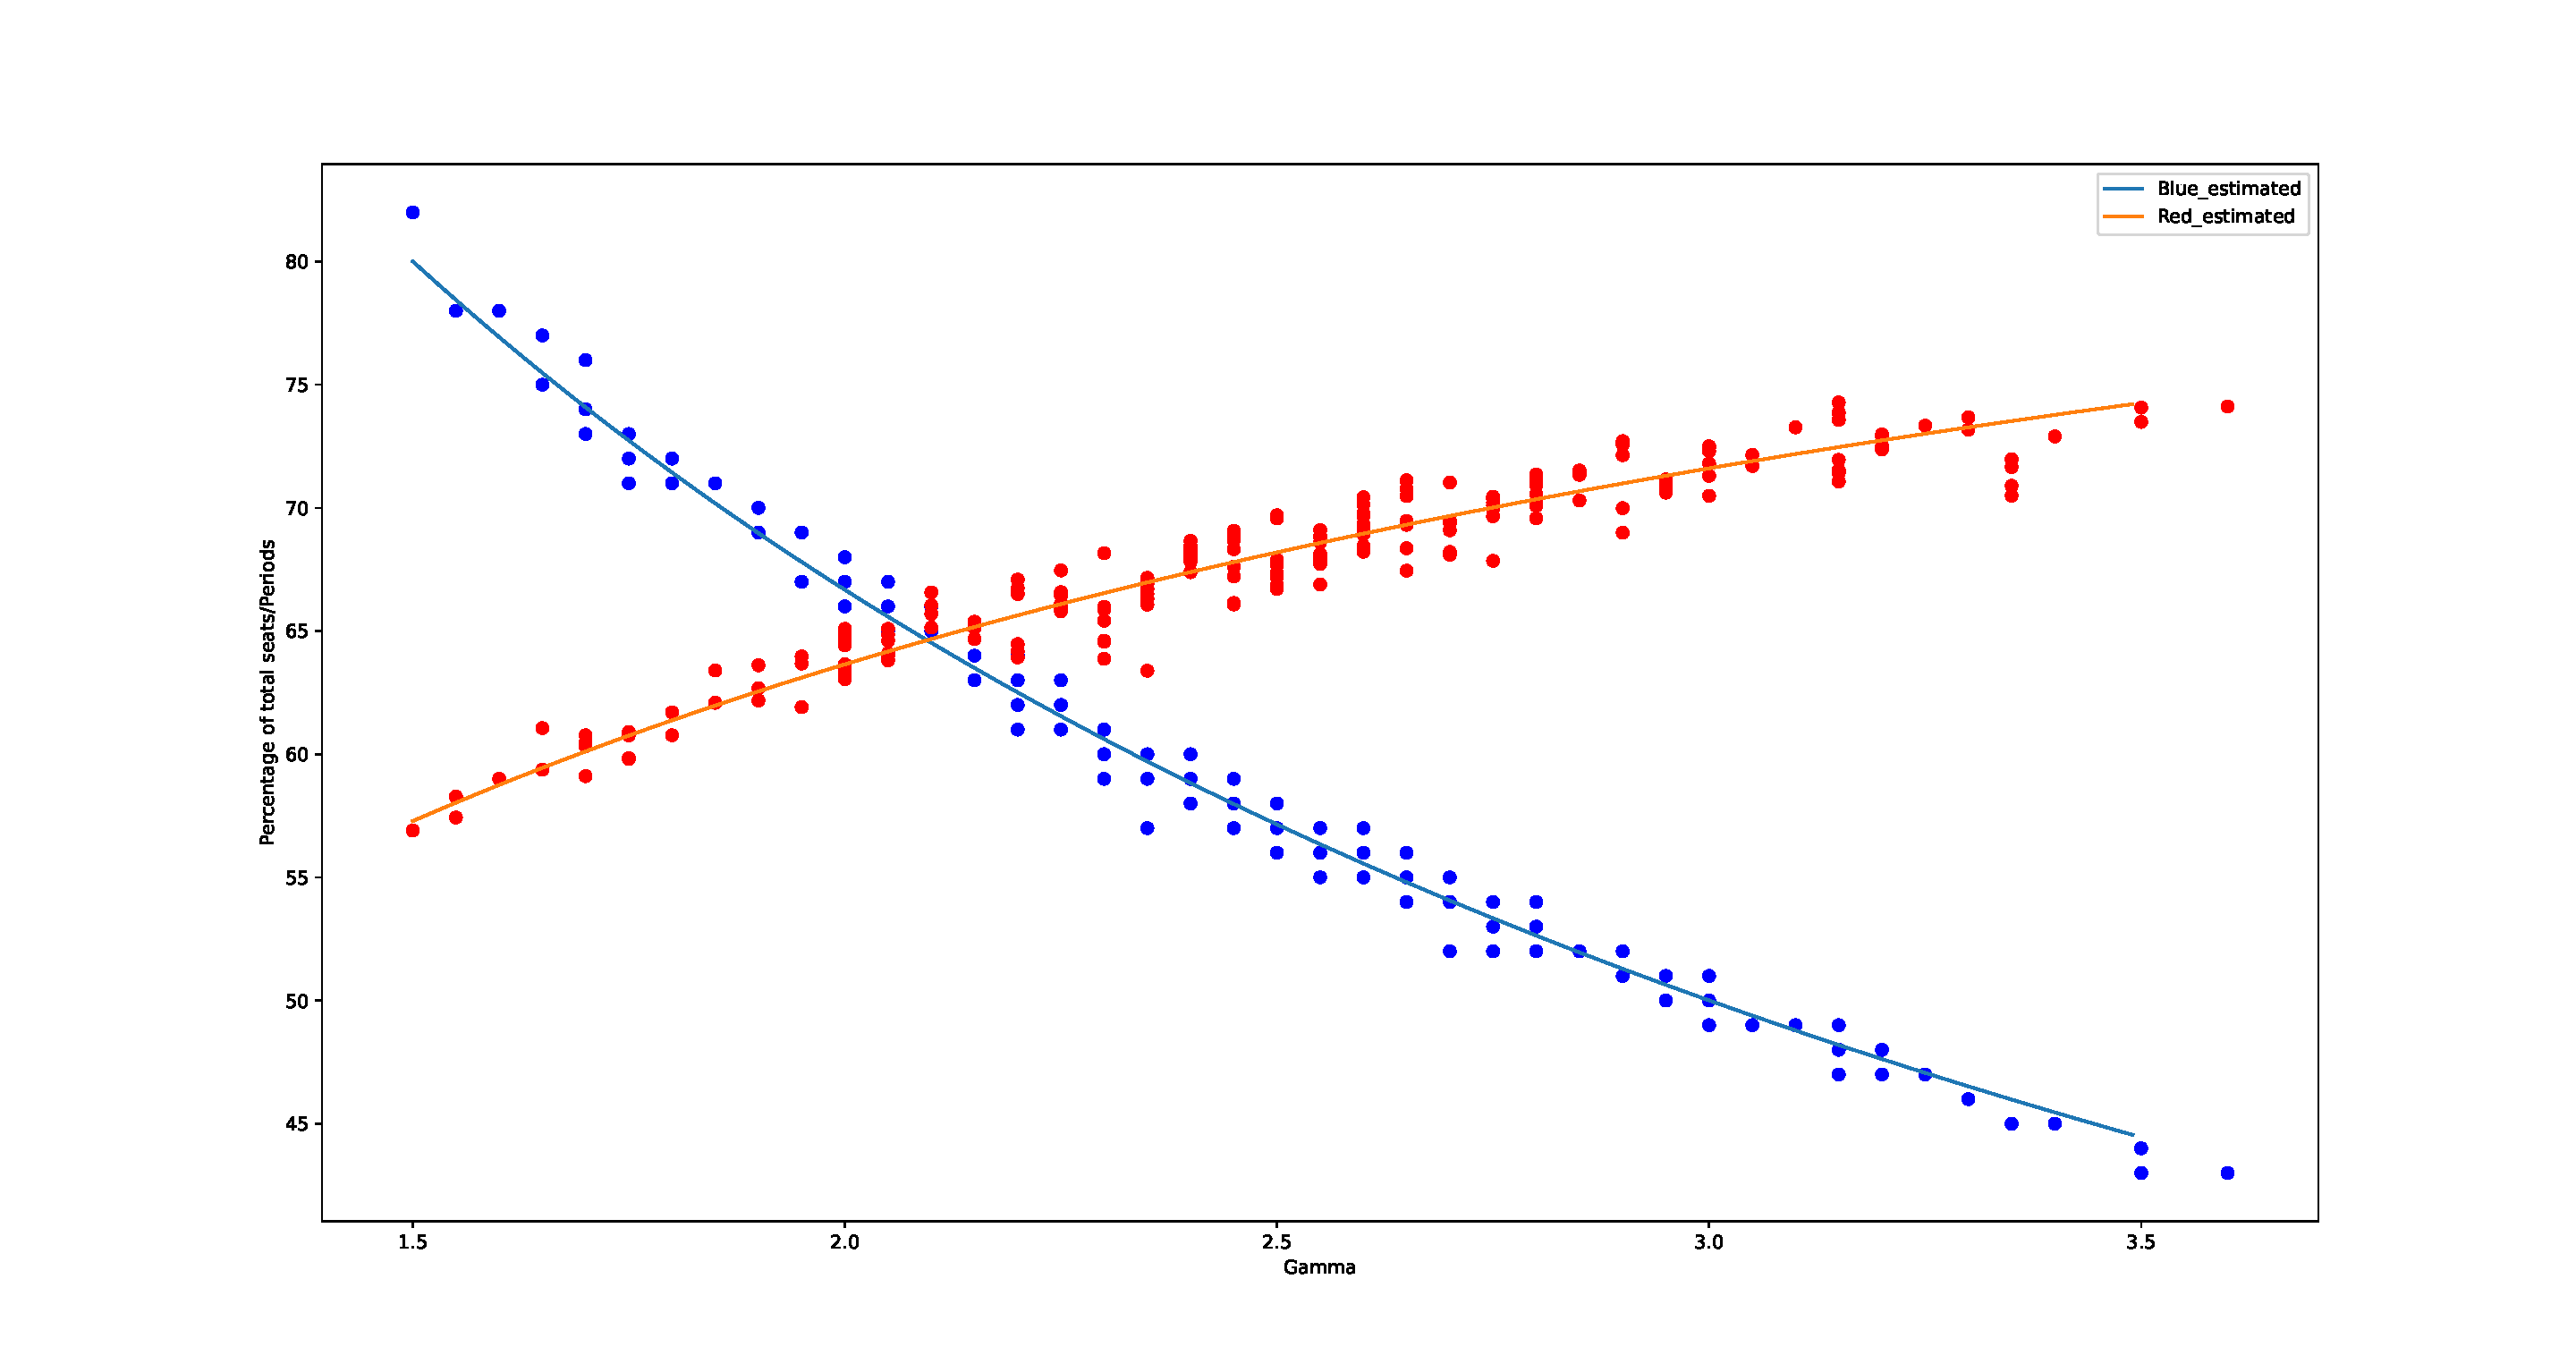
\includegraphics[width=0.8\textwidth]{./Figures/gamma_estimation.pdf}
  \caption{Gap points and their estimation under 200 probabilities}
\end{figure}

By examining the relationship between the gap point and the increment of $\gamma$, we can find that $\gamma$ can be used to estimate gap point.

\subsubsection{Impact of Social Distancing as Demands Increase}
Now, we consider impact of social distance as demands increase by changing $T$. Specifically, we consider two situations: $\gamma = 2.5$ and $\gamma = 1.9$. We set the parameters as follows: $T$ varies from 30 to 120, the step size is 1.  The seat layout consists 10 rows and the number of seats per row is 21. The social distancing is 1 seat.

The figure below displays the outcomes of groups who were accepted under two different conditions: with social distancing measures and without social distancing measures. For the former case, we employ SPP to obtain the results. In this case, we consider the constraints of social distancing and optimize the seat allocation accordingly. For the latter case, we adopt a different approach. We simply accept all incoming groups as long as the capacity allows, without considering the constraints of groups needing to sit together. This means that we prioritize filling the available seats without enforcing any specific seating arrangements or social distancing requirements. Since the various probabilities with the same $\gamma$ exhibit similar patterns as shown in the figure, we present only one case of probabilities to illustrate the detailed figure.

\begin{figure}[h]
  \centering
  \subfigure[When $\gamma =2.5$]{
    \label{Fig.sub.1}
    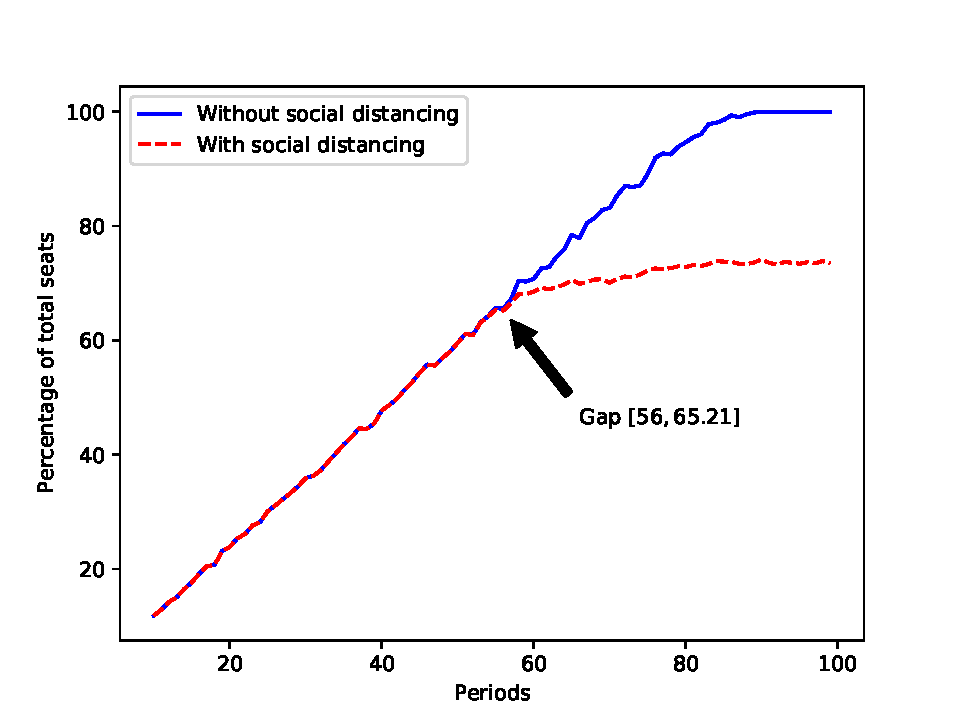
\includegraphics[width=0.48\textwidth]{./Figures/p1.pdf}}
  \subfigure[When $\gamma =1.9$]{
    \label{Fig.sub.2}
    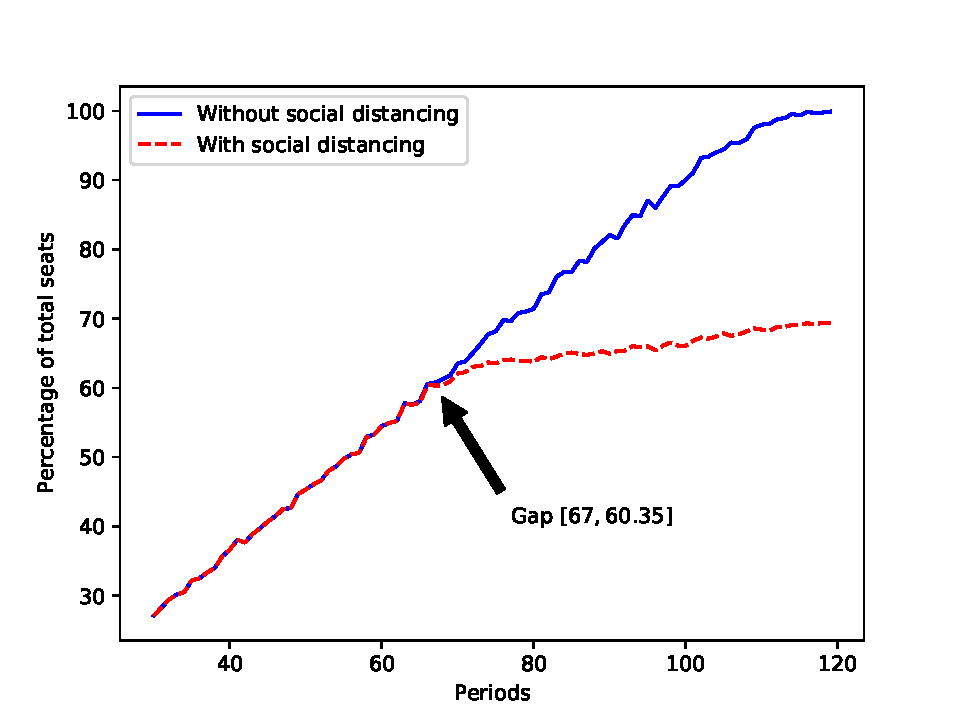
\includegraphics[width=0.48\textwidth]{./Figures/p2.pdf}}
  \caption{The occupancy rate over the number of arriving people}
  \label{Fig.lable}
\end{figure}

The analysis comprises three stages. In the first stage, where the capacity is sufficient, social distancing measures have no impact on the outcome. In the second stage, the gap between the outcomes with and without social distancing measures widens as $T$ increases. Finally, in the third stage, as $T$ continues to increase, the gap between the outcomes with and without social distancing measures converges when both situations accept the maximum number of people.

The table below presents the gap points and the percentage gaps for different demand levels (130, 150, 170, 190, 210).

\begin{table}[]
  \centering
  \caption{Gap points of different gammas and percentage differences under different demands}
\begin{tabular}{lllllll}
  \hline
  \multicolumn{1}{|l|}{\multirow{2}{*}{$\gamma$}} & \multicolumn{1}{l|}{\multirow{2}{*}{gap point}} & \multicolumn{5}{l|}{difference under different demands}   \\ 
  \cline{3-7} 
  \multicolumn{1}{|l|}{}                      & \multicolumn{1}{l|}{}                    & \multicolumn{1}{l|}{130} & \multicolumn{1}{l|}{150} & \multicolumn{1}{l|}{170} & \multicolumn{1}{l|}{190} & \multicolumn{1}{l|}{210} \\ 
  \hline
  \multicolumn{1}{|l|}{1.9}  & \multicolumn{1}{l|}{[69, 65.52]}  & \multicolumn{1}{l|}{0.25}  & \multicolumn{1}{l|}{5.82}  & \multicolumn{1}{l|}{12.82} & \multicolumn{1}{l|}{20.38} & \multicolumn{1}{l|}{24.56} \\ 
  \hline                                    
  \multicolumn{1}{|l|}{2.1}  & \multicolumn{1}{l|}{[64, 67.74]}  & \multicolumn{1}{l|}{0.05}  & \multicolumn{1}{l|}{4.11}  & \multicolumn{1}{l|}{11.51} & \multicolumn{1}{l|}{18.77} & \multicolumn{1}{l|}{21.87} \\ 
  \hline           
  \multicolumn{1}{|l|}{2.3}  & \multicolumn{1}{l|}{[61, 69.79]}  & \multicolumn{1}{l|}{0}  & \multicolumn{1}{l|}{2.29}  & \multicolumn{1}{l|}{10.21} & \multicolumn{1}{l|}{17.36} & \multicolumn{1}{l|}{21.16} \\ 
  \hline           
  \multicolumn{1}{|l|}{2.5}  & \multicolumn{1}{l|}{[57, 70.89]}  & \multicolumn{1}{l|}{0}  & \multicolumn{1}{l|}{1.45}  & \multicolumn{1}{l|}{9.30} & \multicolumn{1}{l|}{15.78} & \multicolumn{1}{l|}{19.80} \\ 
  \hline          
  \multicolumn{1}{|l|}{2.7}  & \multicolumn{1}{l|}{[53, 71.28]}  & \multicolumn{1}{l|}{0}  & \multicolumn{1}{l|}{1.38}  & \multicolumn{1}{l|}{7.39} & \multicolumn{1}{l|}{14.91} & \multicolumn{1}{l|}{19.14} \\ 
  \hline            
\end{tabular}
\end{table}

According to Lemma \ref{lem_pattern}, when the largest pattern is assigned to each row, the resulting occupancy rate is $\frac{16}{20} = 80\%$, which is the upper bound of occupancy rate. The maximum number of people that can be accepted is $200 * \frac{16}{20} = 160$, which is the upper bound on the number of people that can be accepted.


% \subsection{Comparison of Different Probabilities When Supply and Demand Are Close}
% When we set the number of periods $T$ to be equal to $T'$, representing a state where the expected demand and supply are in balance, we can observe differences among the outcomes for different probabilities.

% We sample $p_1$, $p_2$, and $p_3$ from 0.05 to 0.95 with an increment of 0.05. The seat layout still remains the same as the above experiments. The figure below shows the number of people served for each value of $\gamma$. For each probability combination, the blue point represents the average number of people served over 50 instances, and the red point represents the estimated number of people served. 

% \begin{figure}[h]
%   \centering
%   \subfigure[One instance for each probability combination]{
%     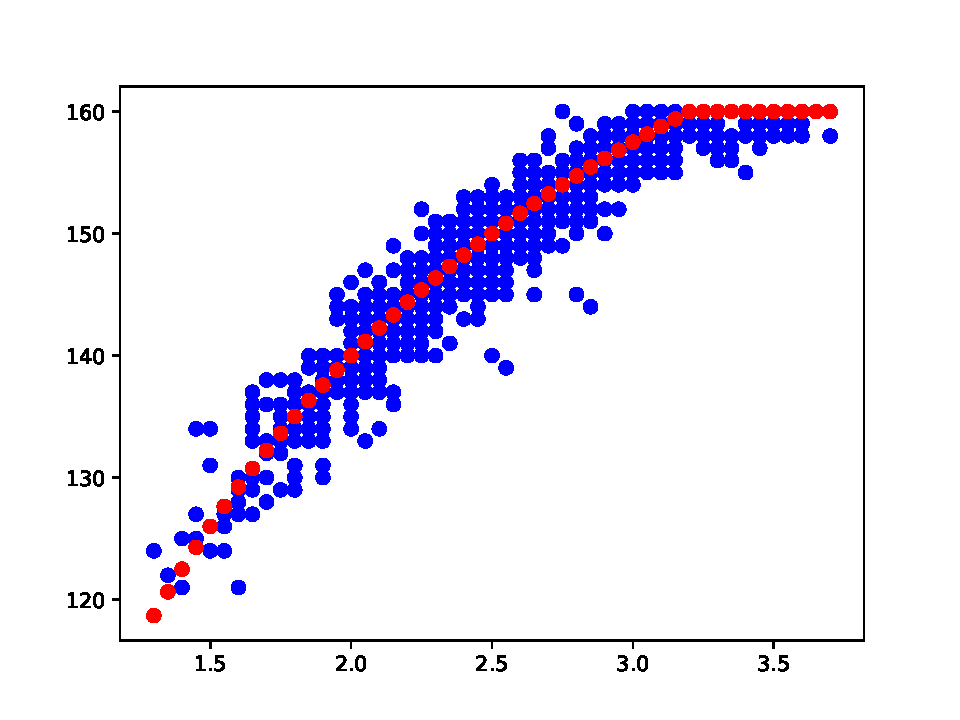
\includegraphics[width=0.48\textwidth]{./Figures/diff_1.pdf}}
%   \subfigure[Average of 50 instances for each probability combination]{
%     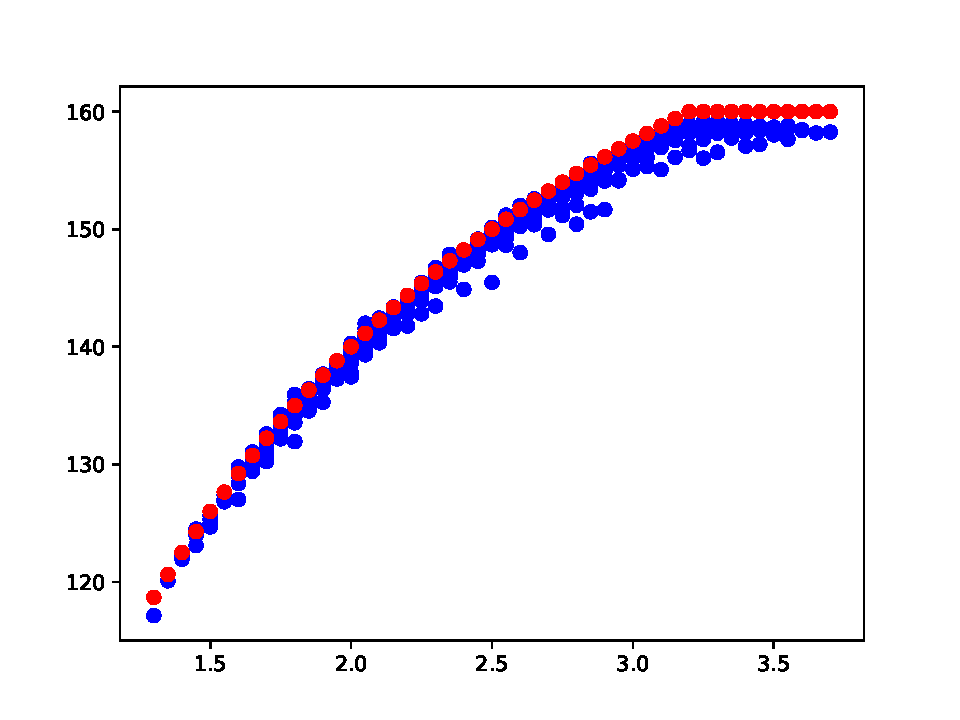
\includegraphics[width=0.48\textwidth]{./Figures/diff_2.pdf}}
%   \caption{The number of people accepted versus $\gamma$}
% \end{figure}

% If the largest pattern is assigned to each row, the resulting occupancy rate is $\frac{16}{21}$. The maximum number of people that can be accepted is $200 * \frac{16}{20} = 160$, which is the upper bound on the number of people that can be accepted. The estimated number of people accepted is given by $\frac{\gamma}{\gamma+1} * 200$, as indicated by the red points in the figure.

% \subsubsection{Analysis on The Difference Between Blue and Red Points}
% We can give the absolute difference between the blue point and red point for each probability combination as below.

% \begin{table}[ht]
%   \centering
%   \caption{Absolute Difference Proportion}\label{tab_diff}
%   \begin{tabular}{|l|l|l|l|l|}
%   \hline
%   \# of instances & abs\_diff $\geq$ 1 & abs\_diff $\geq$ 2 & abs\_diff $\geq$ 3 & abs\_diff $\geq$ 4 \\
%   \hline
%   20 & 32.92 \% & 5.13 \% & 1.74\% & 0.51 \% \\
%   50 & 22.46 \% & 4.31 \% & 1.54 \% & 0.31 \%  \\
%   100 & 20.00 \% & 4.21 \% & 1.54 \% & 0.31 \% \\
%   \hline
%   \end{tabular}
% \end{table}

% \begin{figure}[ht]
%   \centering
%   \subfigure[Average of 50 instances for each probability combination]{
%     \label{Fig1}
%     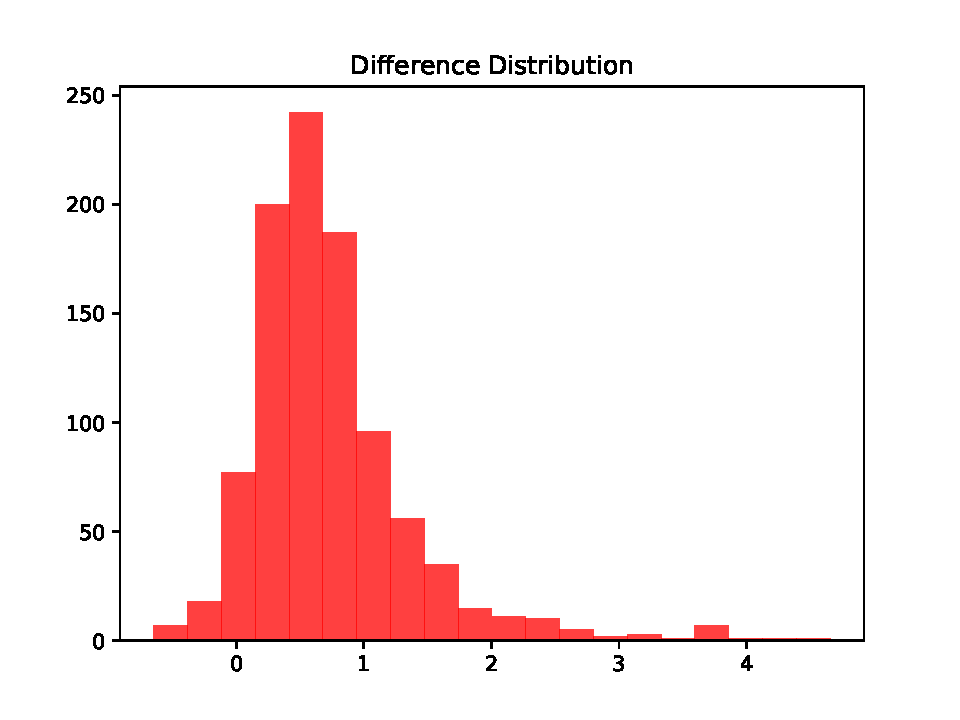
\includegraphics[width=0.48\textwidth]{./Figures/Figure_50.pdf}}
%   \subfigure[Average of 100 instances for each probability combination]{
%     \label{Fig2}
%     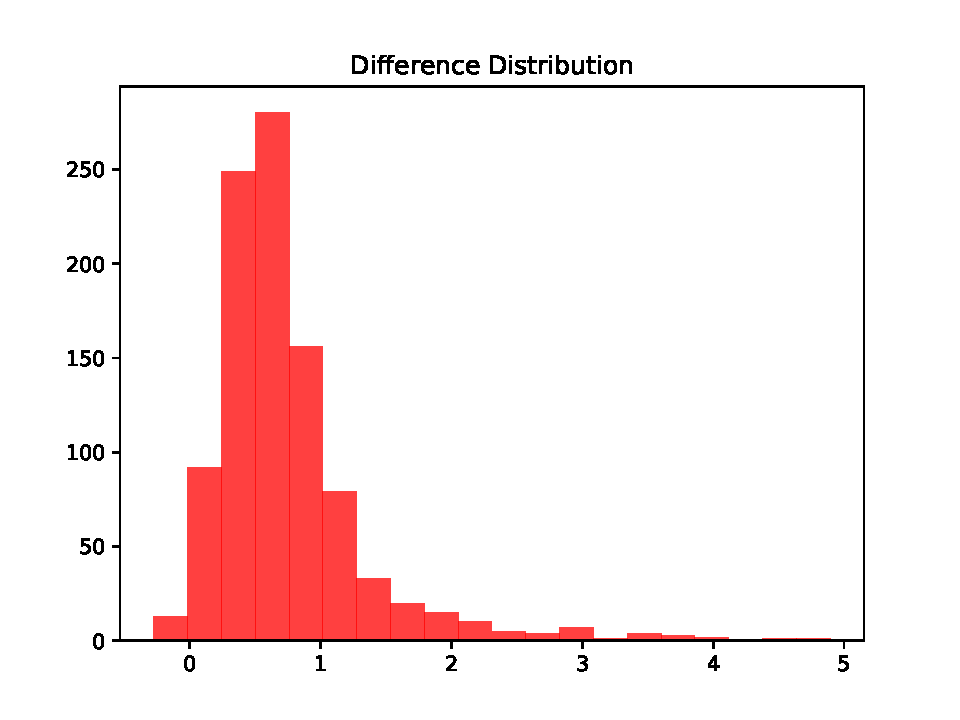
\includegraphics[width=0.48\textwidth]{./Figures/Figure_100.pdf}}
%   \caption{The difference distribution}
%   \label{fig_diff}
% \end{figure}

% Table \ref{tab_diff} displays the absolute difference proportion for the average of 20, 50, and 100 instances, while Figure \ref{fig_diff} shows the difference distribution for the average of 50 and 100 instances. These results suggest that we can estimate the attendance rate based on $\gamma$ for most probability combinations.

% However, we have also observed that some blue points in the figure are significantly distant from their corresponding red points. This is evident when the probability combination is $[0.05, 0.05, 0.85, 0.05]$ (which corresponds to $\gamma = 2.9$), and the demands cannot be accommodated by constructing full patterns for every row, which does not satisfy our assumption. This leads to a considerable gap between the blue and red points in this case. For example, the demands could be $[4, 1, 45, 2]$ or $[2, 2, 47, 1]$ according to the probability combination, but the typical pattern that can be generated is $(4,4,4,4)$, which is not full.


% % \begin{table}[ht]
% %   \centering
% %   \caption{Gap points and gap percentage of different probabilities}
% %   \begin{tabular}{|l|l|l|}
% %   \hline
% %   $\gamma$  & gap point & gap percentage \\
% %   \hline
% %   $[1.5,1.7]$   & [56, ] & [65.21, ] \\
% %   $[1.7,1.9]$   & [56, ] & [65.21, ] \\
% %   $[1.9,2.1]$   & [56, ] & [65.21, ] \\
% %   $[2.1,2.3]$   & [56, ] & [65.21, ] \\
% %   $[2.1,2.3]$   & [56, ] & [65.21, ] \\
% %   \hline
% %   \end{tabular}
% % \end{table}


% % For each $\gamma$, we give several probabilities in the table. We can find the actual gap points with the same $\gamma$ are close.

% % \begin{table}[ht]
% %   \centering
% %   \caption{Actual Gap points of different probabilities}
% %   \begin{tabular}{|l|l|l|l|}
% %   \hline
% %   $\gamma$  & probabilities & gap point & gap percentage \\
% %   \hline
% %   2.5  & [0.25,0.25,0.25,0.25] & 56 & 65.21 \\
% %   2.5  & [0.1,0.4,0.4,0.1] & 55 & 65.59 \\
% %   2.5  & [0.1, 0.5, 0.2, 0.2] & 55 & 65.45 \\
% %   2.5  & [0.2, 0.3, 0.3, 0.2] & 54 & 64.56 \\
% %   2.5  & [0.3, 0.2, 0.2, 0.3] & 55 & 65.51\\
% %   2.5  & [0.2, 0.4, 0.1, 0.3] & 55 & 65.41 \\
% %   1.9  & [0.4, 0.4, 0.1, 0.1] & 67 & 60.35 \\
% %   1.9  & [0.5, 0.2, 0.2, 0.1] & 67 & 58.9  \\
% %   1.9  & [0.3, 0.5, 0.2, 0]  &  68 & 61.7  \\
% %   1.9  & [0.6, 0.1, 0.1, 0.2] & 66 & 58.31 \\
% %   \hline
% %   \end{tabular}
% % \end{table}


% % \subsubsection{Results of Different Seat Layouts}
% % If we modify the even seat layout, the differences between the red and blue points will decrease, and some outliers may be eliminated. To maintain the same total seating capacity, we compare two layouts with the even seat layout. The step-size seat layout consists of rows with 17, 18, 19, 20, 21, 21, 22, 23, 24, and 25 seats, while the random seat layout has rows with 19, 20, 21, 21, 23, 24, 26, 17, 19, and 20 seats. Both layouts can accommodate a maximum of 164 people when each row corresponds to the largest pattern.

% % \begin{figure}[ht]
% %   \centering
% %   \subfigure[Average of 50 instances for step-size seat layout]{
% %     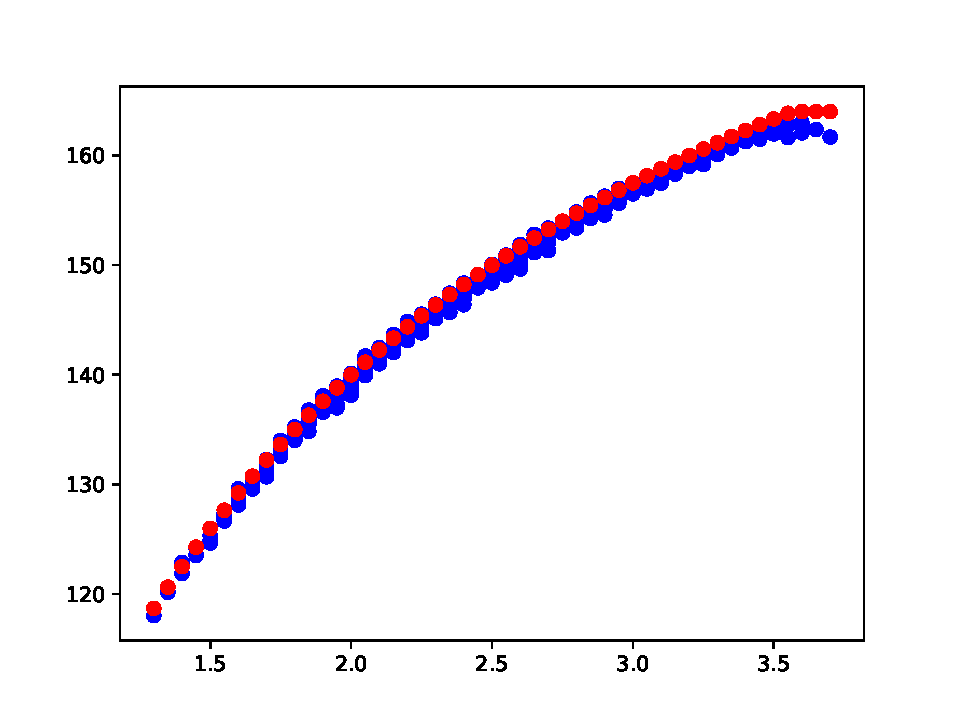
\includegraphics[width=0.48\textwidth]{./Figures/stepsize_seat.pdf}}
% %   \subfigure[Average of 50 instances for random seat layout]{
% %     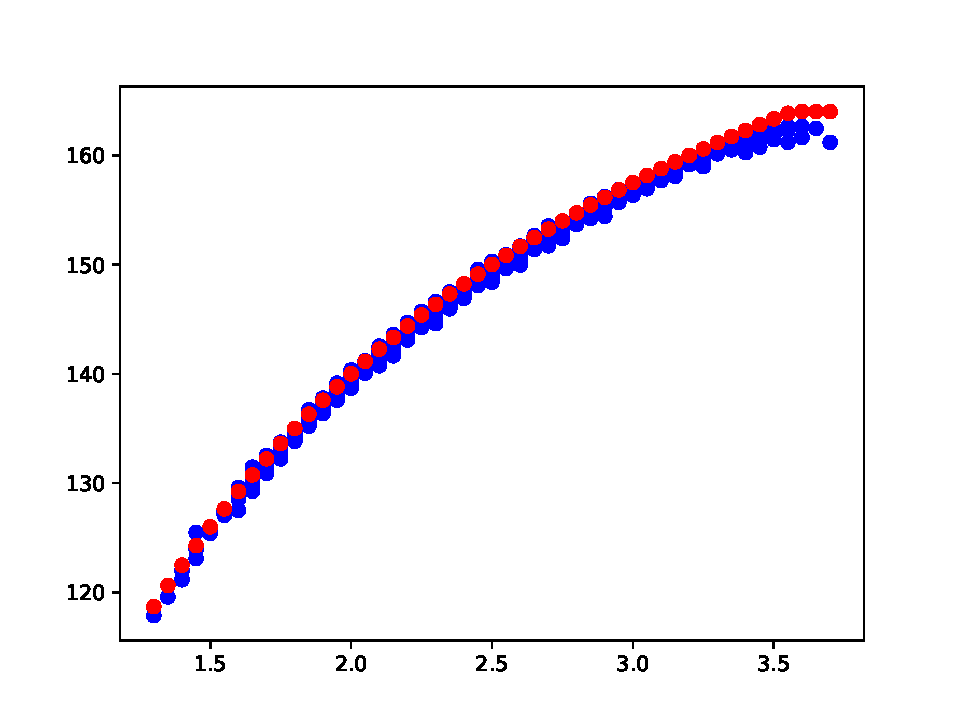
\includegraphics[width=0.48\textwidth]{./Figures/random_seat.pdf}}
% %   \caption{The number of people served versus $\gamma$}
% % \end{figure}

% % The results suggest that a random seat layout may provide a more accurate estimation, implying that such a layout is more capable of accommodating uncertain demands and achieving a full pattern that can accept more people.

% % % When $p = [0.25, 0.25, 0.25, 0.25]$, $E(D) = 2.5 T$. Let $p_1*1 + p_2*2 + p_3*3 + p_4*4 = 2.5$, 
% % % Let $E(D) = 150, T = 50, 60, 75$. The number of seats: 200, 210, 225.


% % \newpage

% % % In addition, we evaluate two policies for seat assignment after all group arrivals: one is based on dynamic programming (DP) and the other is based on first-come, first-served (FCFS) scheduling.
% % % We present the results of our experiments and discuss their implications.


% \subsection{Measurement}
% Suppose a real scenario with a fixed sequence, $s^{r}$. Solving the following program can obtain the optimal value, $V_{s^{r}}$. (Offline)

% Then the difference is $V_{s^{r}} - \text{our result}$.

% WS(the value under wait-and-see policy with all possible scenarios)

% EVPI(Expected Value of Perfect Information) = WS - the value of deterministic equivalent form
